\section{Experimental results}
\label{sec:experiments}

We conducted our experiments using Amazon Mechanical
Turk~\footnote{http://www.mturk.com}, which allows workers (our pool
of prospective subjects) to perform small jobs for a fee through a Web
interface.  No specialized training or knowledge is typically expected
of the workers.  Amazon Mechanical Turk has been successfully used in
the past to develop gold-standard data for natural language
processing~\cite{snow-08} and to label images~\cite{imagenet-cvpr09}.

we prepare two randomly-chosen, 100-document subsets of English
Wikipedia~\footnote{http://en.wikipedia.org}.  For convenience, we
denote these two sets of documents as \emph{set1} and \emph{set2}.
For each document, we keep only the first 150 words for our
experiments.  Because of the encyclopedic nature of the corpus, the
first 150 words typically provides a broad overview of the themes in
the article.  We also removed from the corpus stop words and words
which occur infrequently\footnote{Infrequently occurring words were
  identified as those appearing fewer than eight times on a larger
  collection of 7726 articles.}, leading to a lexicon of 8263 words.
After this pruning \emph{set1} contained 11614 words and \emph{set2}
contained 11318 words.

Workers were asked to perform twenty of the taggings described in
\mysec{sec:tasks} for each task; workers were paid \$0.25 for each
such task.  The number of latent topics, $K$, is a free parameter.
Here we explore two values of this parameter, $K=10$ and $K=15$,
leading to a total of four experiments --- two for each set of
documents and two for each value of $K$.

\subsection{Tagging behavior}

There are several metrics commonly used to evaluate topic models in
the literature~\cite{wallach-09}.  Many of these metrics are
\emph{predictive} metrics; that is, they capture the model's ability
to predict a \emph{test set} of unseen documents after having learned
its parameters from a \emph{training set}.  In this work, we set aside
20\% of the documents in each corpus as a test set and train on the
remaining 80\% of documents.  We then compute predictive rank and
predictive log likelihood.

\begin{table*}
  \caption{The five words with the highest probability mass in each topic inferred by humans using the task described in \mysec{sec:tasks}.  Each subtable shows the results for a particular experimental setup.   Each row is a topic; the most probable words are ordered from left to right.}
\label{tab:topic-samples}
\centering
\footnotesize
\hspace*{-.4in}
\subfigure[\emph{set1}, $K = 10$]{
\begin{tabular}{lllll}
  railway & lighthouse & rail & huddersfield & station \\ 
  school & college & education & history & conference \\ 
  catholic & church & film & music & actor \\ 
  runners & team & championships & match & racing \\ 
  engine & company & power & dwight & engines \\ 
  university & london & british & college & county \\ 
  food & novel & book & series & superman \\ 
  november & february & april & august & december \\ 
  paint & photographs & american & austin & black \\ 
   war & history & army & american & battle \\ 
\end{tabular}
}%
\subfigure[\emph{set2}, $K = 10$]{
  \begin{tabular}{|lllll}
    president & emperor & politician & election & government \\ 
    american & players & swedish & team & zealand \\ 
    war & world & navy & road & torpedo \\ 
    system & pop & microsoft & music & singer \\ 
    september & 2007 & october & december & 1999 \\ 
    television & dog & name & george & film \\ 
    people & malay & town & tribes & cliff \\ 
    diet & chest & enzyme & hair & therapy \\ 
    british & city & london & english & county \\ 
    school & university & college & church & center \\ 
  \end{tabular}
}
\hspace*{-.5in}
\subfigure[\emph{set1}, $K = 15$]{
\begin{tabular}{lllll}
australia & knee & british & israel & set \\ 
  catholic & roman & island & village & columbia \\ 
  john & devon & michael & austin & charles \\ 
  school & university & class & community & district \\ 
  november & february & 2007 & 2009 & 2005 \\ 
  lighthouse & period & architects & construction & design \\ 
  railway & rail & huddersfield & ownership & services \\ 
  cyprus & archdiocese & diocese & king & miss \\ 
  carson & gordon & hugo & ward & whitney \\ 
  significant & application & campaign & comic & considered \\ 
  born & london & american & england & black \\ 
  war & defense & history & military & artillery \\ 
  actor & film & actress & band & designer \\ 
  york & michigan & florida & north & photographs \\ 
  church & catholic & county & 2001 & agricultural \\ 
\end{tabular}
}%
\subfigure[\emph{set2}, $K = 15$]{
\begin{tabular}{|lllll}
  music & pop & records & singer & artist \\ 
  film & paintings & movie & painting & art \\ 
  school & university & english & students & british \\ 
  drama & headquarters & chess & poet & stories \\ 
  family & church & sea & christmas & emperor \\ 
  dog & broadcast & television & bbc & breed \\ 
  champagne & regular & character & characteristic & common \\ 
  election & government & parliament & minister & politician \\ 
  enzyme & diet & protein & hair & oxygen \\ 
  war & navy & weapons & aircraft & military \\ 
  september & october & december & 2008 & 1967 \\ 
  district & town & marin & america & american \\ 
  car & power & system & device & devices \\ 
  hockey & players & football & therapy & champions \\ 
  california & zealand & georgia & india & kolkata \\ 
\end{tabular}
}
\vspace{0.2in}
\end{table*}

\begin{figure*}
\centering
\subfigure[$K = 10$]{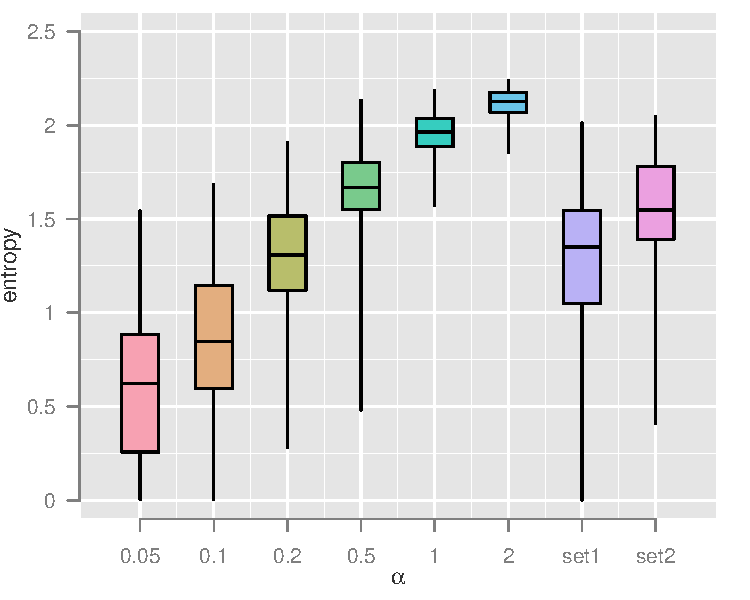
\includegraphics[width = .47\linewidth]{figures/entropy_K10}}%
\subfigure[$K = 15$]{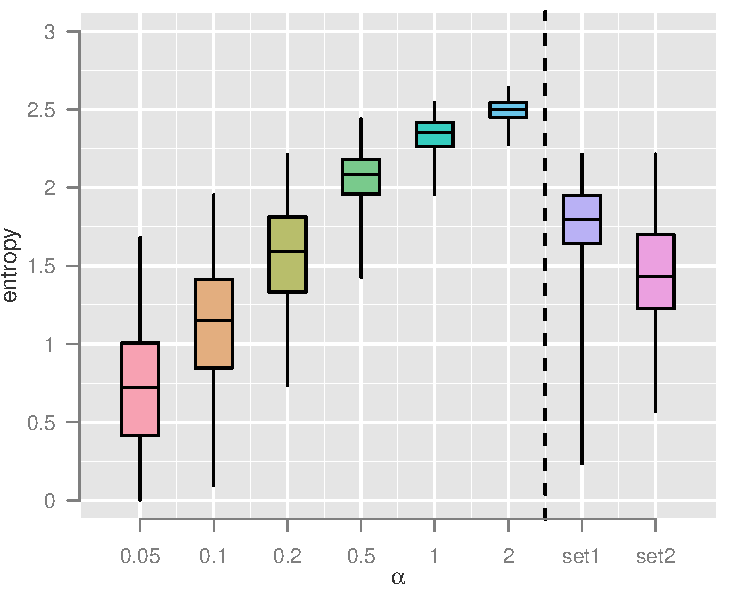
\includegraphics[width = .47\linewidth]{figures/entropy_K15}}

\caption{A comparison of the entropy of distributions drawn from a
  Dirichlet versus the entropy of the topic proportions inferred by
  workers.  Each column of the boxplot shows the distribution of
  entropies for 100 draws from a Dirichlet distribution with parameter
  $\alpha$.  The two rightmost columns show the distribution of the
  entropy of the topic proportions inferred by workers on \emph{set1}
  and \emph{set2}.  The $\alpha$ workers typically falls between 0.2
  and 0.5.}

\label{fig:entropy}
\end{figure*}

\subsection{Comparison with LDA}
\begin{figure*}
\centering
\subfigure[\emph{full}, $K = 10$]{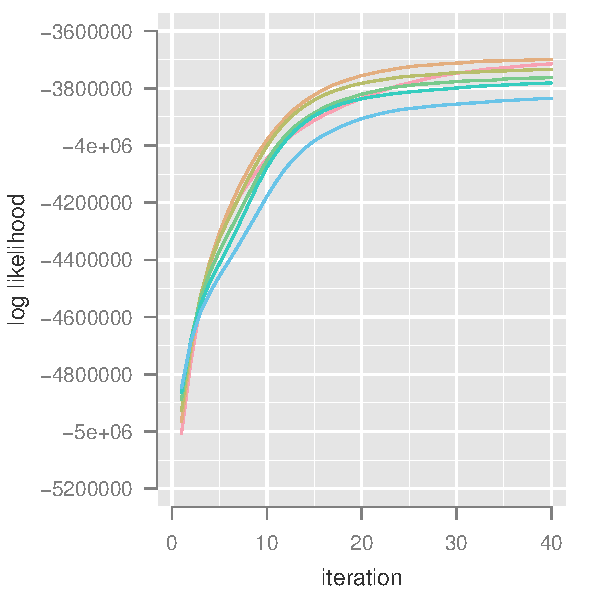
\includegraphics[width = .32\linewidth]{figures/lda_ll_full_10}}%
\subfigure[\emph{set1}, $K = 10$]{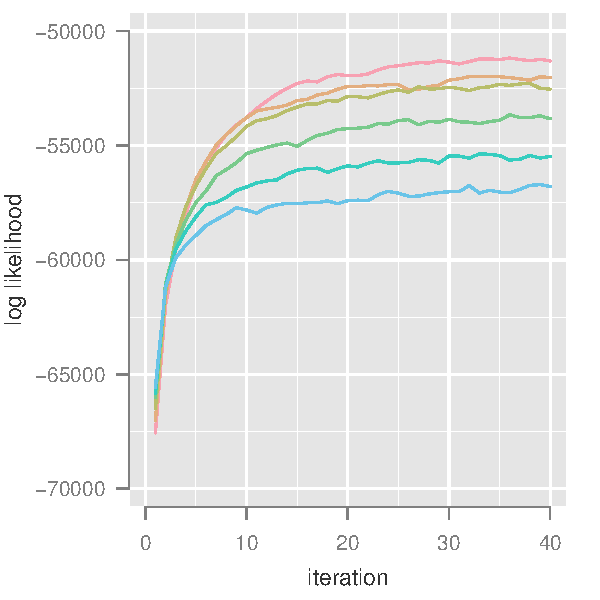
\includegraphics[width = .32\linewidth]{figures/lda_ll_set1_10}}%
\subfigure[\emph{set2}, $K = 10$]{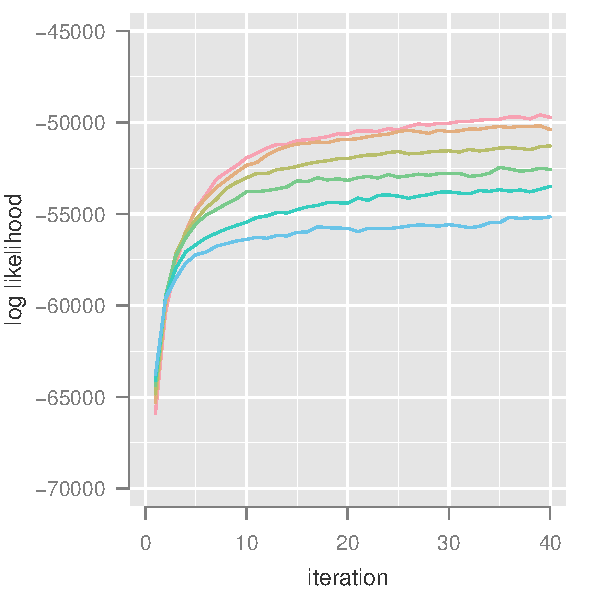
\includegraphics[width = .32\linewidth]{figures/lda_ll_set2_10}}

\subfigure[\emph{full}, $K = 15$]{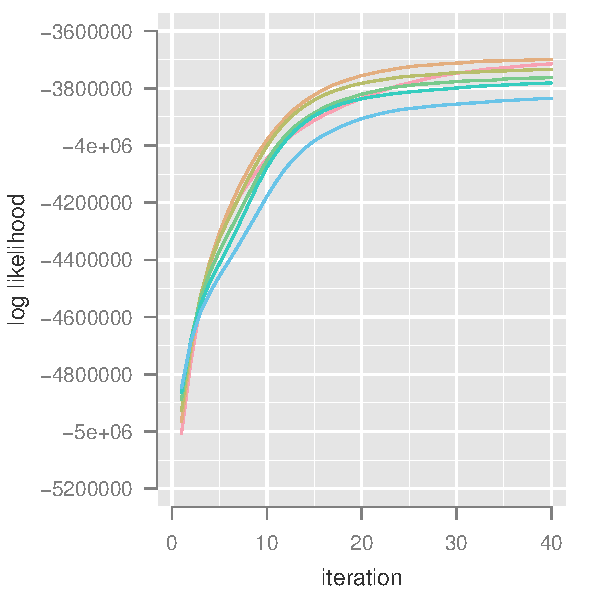
\includegraphics[width = .32\linewidth]{figures/lda_ll_full_10}}%
\subfigure[\emph{set1}, $K = 15$]{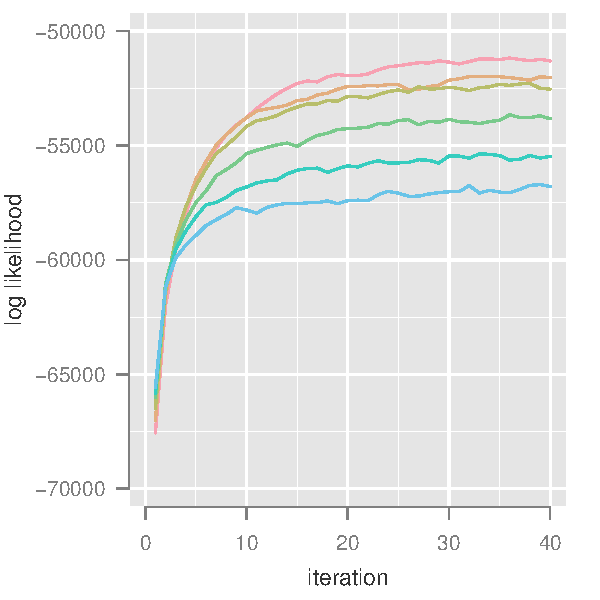
\includegraphics[width = .32\linewidth]{figures/lda_ll_set1_10}}%
\subfigure[\emph{set2}, $K = 15$]{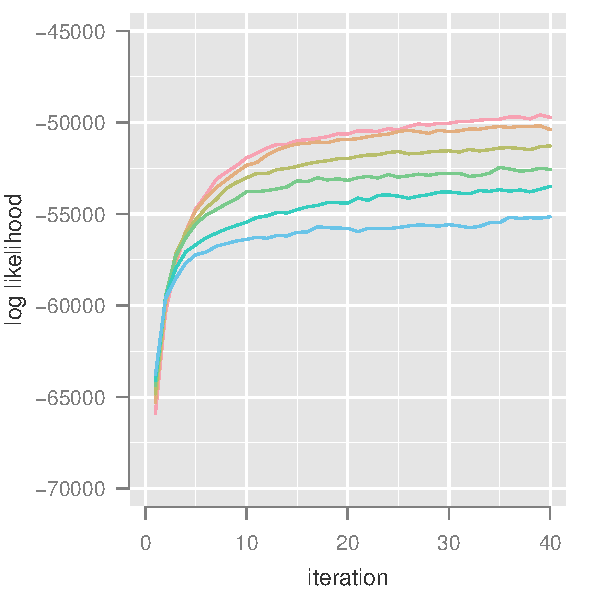
\includegraphics[width = .32\linewidth]{figures/lda_ll_set2_10}}

\caption{The log-likelihood achieved by LDA as a function of iteration.  \emph{full} refers to a larger set of 7726 Wikipedia articles.   There is one series for each value of $\alpha \in \{0.05, 0.1, 0.2, 0.5, 1.0, 2.0\}$ from top to bottom.}
\label{fig:ll}
\end{figure*}

\begin{table*}[ht]
\footnotesize
\centering
  \caption{The five words with the highest probability mass in each topic inferred by LDA.  Each subtable shows the results for a particular experimental setup.   Each row is a topic; the most probable words are ordered from left to right.}
\label{tab:lda-topic-samples}
\hspace*{-.1in}
\subfigure[\emph{set1}, $K=10$]{
\begin{tabular}{lllll}
born & 2004 & team & award & sydney \\ 
  regiment & army & artillery & served & scouting \\ 
  line & station & main & island & railway \\ 
  region & street & located & site & knee \\ 
  food & february & conference & day & 2009 \\ 
  pride & greek & knowledge & portland & study \\ 
  catholic & church & roman & black & time \\ 
  class & series & film & actor & engine \\ 
  travel & human & office & management & defense \\ 
  school & born & war & world & university \\ 
\end{tabular}
}%
\subfigure[\emph{set2}, $K=10$]{
\begin{tabular}{|lllll}
september & english & edit & nord & hockey \\ 
  black & hole & current & england & model \\ 
  training & program & war & election & navy \\ 
  school & university & district & city & college \\ 
  family & word & international & road & japan \\ 
  publication & time & day & india & bridge \\ 
  born & pop & world & released & march \\ 
  won & video & microsoft & project & hungary \\ 
  film & hair & bank & national & town \\ 
  people & name & french & therapy & artist \\ 
\end{tabular}
}
\hspace*{-.3in}
\subfigure[\emph{set1}, $K=15$]{
\begin{tabular}{lllll}
time & michael & written & experience & match \\ 
  line & station & railway & branch & knowledge \\ 
  film & land & pass & set & battle \\ 
  william & florida & carson & virginia & newfoundland \\ 
  war & regiment & british & army & south \\ 
  reaction & terminal & copper & running & complex \\ 
  born & school & world & college & black \\ 
  food & conference & flight & medium & rail \\ 
  township & scouting & census & square & county \\ 
  travel & defense & training & management & edges \\ 
  series & actor & engine & november & award \\ 
  pride & portland & band & northwest & god \\ 
  team & knee & 2004 & sydney & israel \\ 
  catholic & located & site & region & church \\ 
  class & february & time & public & king \\ 
\end{tabular}
}%
\subfigure[\emph{set2}, $K=15$]{
\begin{tabular}{|lllll}
family & protein & enzyme & acting & oxygen \\ 
  england & producer & popular & canadian & sea \\ 
  system & death & artist & running & car \\ 
  character & series & dark & main & village \\ 
  english & word & publication & stream & day \\ 
  training & program & hair & students & electrical \\ 
  district & town & city & local & kolkata \\ 
  september & edit & music & records & recorded \\ 
  black & pop & bank & usually & hole \\ 
  people & choir & road & diet & related \\ 
  war & built & navy & british & service \\ 
  center & million & cut & champagne & players \\ 
  born & television & current & drama & won \\ 
  school & university & college & election & born \\ 
  film & nord & played & league & hockey \\ 
\end{tabular}
}
\end{table*}

As described in \mysec{sec:wordintrusion}, the word intrusion task
measures how well the inferred topics match human concepts (using
\emph{model precision}, i.e., how well the intruders detected by the
subjects correspond to those injected into ones found by the topic
model).

\myfig{fig:precision} shows boxplots of the precision for the three
models on the two corpora.  In most cases LDA performs best. Although
CTM gives better predictive results on held-out likelihood, it does
not perform as well on human evaluations. This may be because CTM
finds correlations between topics and correlations within topics are
confounding factors; the intruder for one topic might be selected from
another highly correlated topic.  The performance of pLSI degrades
with larger numbers of topics, suggesting that
overfitting~\cite{blei-03} might affect interpretability as well as
predictive power.

\myfig{fig:topic_precision} (left) shows examples of topics with high
and low model precisions from the NY Times data fit with LDA using 50
topics. In the example with high precision, the topic words all
coherently express a painting theme.  For the low precision example,
``taxis'' did not fit in with the other political words in the topic,
as $87.5\%$ of subjects chose ``taxis'' as the intruder.



